\chapter{Гидродинамическое описание системы}
\label{cha:design}

Перейдем теперь к более грубому, гидродинамическому описанию системы. Для начала нужно определить возможность такого перехода
в рассматриваемой нами системе. Через $L$ обозначим линейный размер всей системы в целом. Для кинетического описания нам было достаточно
что линейные размеры частиц $\sigma$ были намного меньше размера всей системы, т.е. выполнение условия $\sigma\ll L$. Соответственно
все кинетические уравнения пишутся на уровне детализации $\sigma$. Однако гидродинамическое описание происходит на другом уровне,
который мы обозначим $\ell$, и который удовлетворяет условию $\sigma\ll\ell\ll L$. Если мы можем вести изучение системы в таком масштабе,
то можно говорить что мы рассматриваем систему в гидродинамическом приближении. Линейные размеры колец Сатурна, т.е. ширина колец,
растягивается примерно на $L\sim 66 000$ км, в то время как размеры самих частиц варьируются в пределах $\sigma\sim 10^{-2}\div 10^2$ см.
Отсюда хорошо видно что можно подобрать такое значение $\ell\sim 1\div 2$ км, в пределах которого гидродинамическое описание системы
будет вполне оправдано. Таким образом, в дальнейшем мы можем говорить что в пределах $\ell$ вокруг координаты $\br$ находится достаточно большое
количество частиц, по которым можно определить макропараметры системы в зависимости от самой координаты $\br$. Перейдем к непосредственным 
определениям самих макропараметров, необходимых для полного гидродинамического описания системы, и написанию уравнений переноса
этих параметров.

\section{Уравнения переноса}

Зная функцию распределения, можно вводить пространственно распределенные параметры, описывающие систему в целом, а не через отдельно
взятые частицы. Такие параметры называются макропараметрами системы. Мы будем вводить их как моменты вектора скорости частиц $\bv$. Так,
нулевой момент, как мы уже ранее определили, дает нам функцию числовой плотности:
\begin{equation}
  n(t,m,\br) = \int f(t,m,\br,\bv)\,d\bv\;,
\end{equation}
либо функцию плотности масс
\begin{equation}
  \rho(t,m,\br) = mn(t,m,\br) = \int mf(t,m,\br,\bv)\,d\bv\;.
\end{equation}
Данная функция читается так: $\rho(t,m,\br)$ -- это масса в единичном объеме участка кольца в координате $\br$ во время $t$, при этом 
масса вещества данного участка кольца равна $m$. Остальные параметры имеют схожий физический смысл.

Первый момент по скорости дает нам функцию плотности импульса
\begin{equation}
  \rho\bu(t,m,\br)=\int m\bv f(t,m,\br,\bv)\,d\bv\;,
\end{equation}
где $\bu$ -- дает нам среднюю скорость участка кольца. Введем понятие локальной скорости частиц
\begin{equation}\label{eq:local_velocity}
  \bc = \bv-\bu(t,m,\br)\;,
\end{equation}
которая показывает скорость (хаотического движения) частиц в системе отсчета движущейся вместе с участком кольца со скоростью $\bu$.
Таким образом введем понятие \emph{гранулярной температуры} системы, по аналогии с термодинамической температурой как второй момент
по скорости
\begin{equation}
  \frac{D}{2}nT(t,m,\br) = \int\frac{m\bc^2}{2}f(t,m,\br,\bv)\,d\bv\;,
\end{equation}
где $D=3$ -- для трехмерной системы, однако мы будем рассматривать двумерную систему $D=2$.
Нам также понадобятся и другие моменты по скорости, которые уже являются тензорными величинами. Во первых, это
тензор \emph{напряжения}:
\begin{equation}
  \Pi_{ij}(t,m,\br)=m\int v_iv_jf(t,m,\br,\bv)\,d\bv\;,
\end{equation}
который можно разделить на две части используя (\ref{eq:local_velocity})
\begin{equation}
  \Pi_{ij}(t,m,\br)=\rho u_iu_j+P_{ij}\;.
\end{equation}
Первая часть является динамической частью тензора напряжения, а вторая часть называется тензором \emph{внутренних напряжений}:
\begin{equation}
  P_{ij}(t,m,\br)=m\int c_ic_jf(t,m,\br,\bv)\,d\bv\;.
\end{equation}
Разделяя далее данный тензор на диагональную и безсверточную части, получаем:
\begin{equation}
  P_{ij} = \delta_{ji}p_{id}+\pi_{ij}\;,\;\;\;\pi_{ii}=0\;,
\end{equation}
где 
\begin{equation}
  p_{id}=\frac{1}{D}\int m\bc^2f(t,m,\br,\bv)\,d\bv=nT\;,
\end{equation}
давление идеального газа. Безсверточная часть тензора $\pi_{ij}$ также называется тензором \emph{вязких напряжений}.

Наконец, введем следующий тензор
\begin{equation}
  Q_{ijk}=m\int c_ic_jc_kf(t,m,\br,\bv)\,d\bv\;,
\end{equation}
или точнее его свертку по двум индексам
\begin{equation}
  q_i=\bq = \frac{1}{2}Q_{ijj} = \int \frac{m\bc^2}{2}c_if(t,m,\br,\bv)\,d\bv\;,
\end{equation}
который называется вектором \emph{потока тепла}.

\section{Подсистема всякой ерунды}

Культурная вставка dot-файлов через утилиту dot2tex (рис.~\ref{fig:fig02}).

\begin{figure}
  \centering
% [width=0.5\textwidth] --- регулировка ширины картинки
  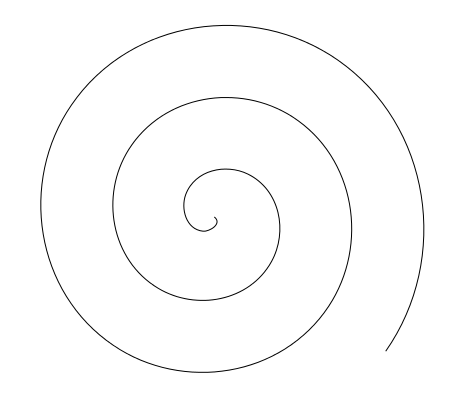
\includegraphics{figures/pic01}
  \caption{Рисунок}
  \label{fig:fig02}
\end{figure}


\subsection{Блок-схема всякой ерунды}

\subsubsection*{Кстати о заголовках}

У нас есть и \Code{subsubsection}. Только лучше её не нумеровать.

%%% Local Variables:
%%% mode: latex
%%% TeX-master: "rpz"
%%% End:
